\chapter{Современное состояние беспилотного транспорта и проблемы его применения} \label{chapt2}

\section{Необходимость применения беспилотного транспорта} \label{sect_Need}

Дорожные происшествия являются самой опасной
угрозой здоровью людей во всем мире. Ущерб от до­рожно­-транспортных 
происшествий (ДТП) превышает
ущерб от всех иных транспортных происшествий (само­летов,
кораблей, поездов, и т. п.) вместе взятых. До­рожно-­транспортные
происшествия являются одной из
важнейших мировых угроз здоровью и жизни людей.
Проблема усугубляется и тем, что пострадавшие в ава­риях — как правило, 
молодые и здоровые (до аварии)
люди. По данным ВОЗ, в мире ежегодно в дорожных
авариях погибают 1,2 млн человек и около 50 млн по­лучают 
травмы. Более 27000 погибает на российских
дорогах, и более 40000 на дорогах США, в пересчете
на количество автомобилей эти цифры означают в год
70 погибших в ДТП на территории России или 15 по­гибших 
в США на каждые 100 000 автомобилей \cite{DTP_ukr}.
% Скопированно без изменений

Известно, что ДТП – непреднамеренное событие, возникающее в результате 
неблагоприятного сочетания факторов в
условиях динамической системы <<человек – автомобиль - дорога>>, вероятность 
которого может увеличиваться под
воздействием неблагоприятных внешних факторов (дождь, гололед, сумерки, дорожные 
работы, т.п.) и следствием
которого является ущерб здоровью человека, повреждение транспортного средства и 
дорожного обустройства.
Факторы, связанные с человеком, транспортным средством и дорожной 
инфраструктурой являются элементами единой
дорожно-транспортной системы, где множество элементов, находящихся в отношениях 
и связях друг с другом,
образуют определенную целостность. Изучение систем требует применения системного 
подхода. Системный подход
нацелен на выявление многообразных типов связей в системе и сведение их в единую 
теоретическую картину.
С точки зрения безопасности дорожного движения интерес для системного изучения 
представляют как сами факторы
риска, так и их различные сочетания, а именно:
\begin{itemize}
  \item человек/автомобиль;
  \item автомобиль/дорога;
  \item дорога/человек.
\end{itemize}

% Эта часть скопирована без изменений

Министерство транспорта Германии в 2002 г. провело исследования причин ДТП 
во многих странах мира. На рисунке \ref{img:dtp_roles} представлена примерная 
картина соотношения данных факторов \cite{DTP_factors}.
% Этот абзац изменен

\begin{figure}[ht] 
  \centering
  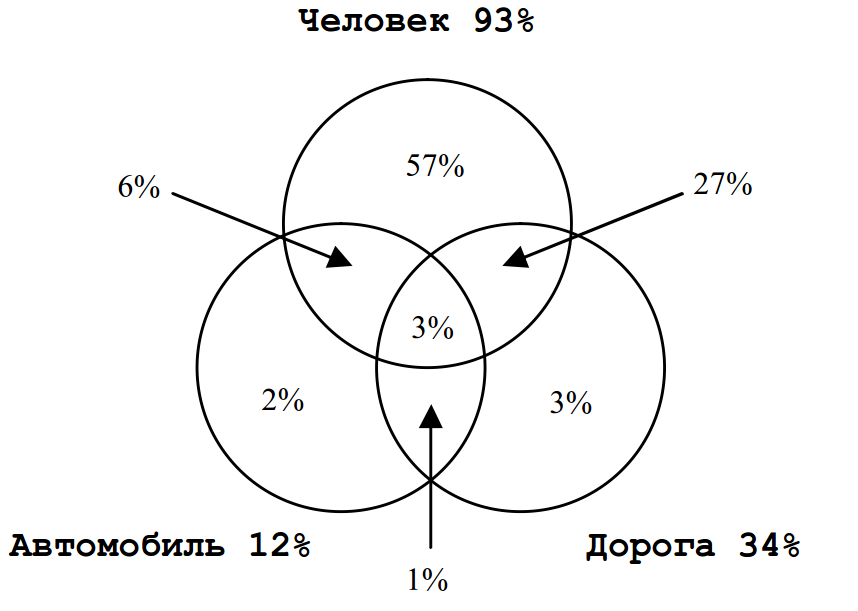
\includegraphics [scale=0.5] {dtp_roles}
  \caption{Роль факторов риска и их сочетаний в возникновении ДТП}
  \label{img:dtp_roles}
\end{figure}

По данной диаграмме можно сделать вывод, что:
\begin{itemize}
  \item главная причина дтп в 57\% случаев – ошибка человека;
  \item еще в 6\% случаев - причиной является проблема взаимодействия человека и 
        автомобиля (например, интерференция навыков в критической ситуации);
  \item еще в 27\% случаев - причиной является проблема взаимодействия человека 
        и дороги (например, провоцирование водителя на превышение скорости 
        посредством прямого и широкого участка дороги за которым следует резкий 
        поворот);
  \item еще в 3\% случаев - причиной является проблема сложного взаимодействия 
        человека, автомобиля и дороги.
\end{itemize}

Таким образом в 93\% случаев ДТП присутствует человеческий фактор, который 
выражается следующими проявлениями:
\begin{enumerate}
  \item Превышение скорости;
    \begin{enumerate}
      \item недостаток опыта для выбора правильной скорости в
            определенных дорожных условиях (мокрое покрытие,
            гололед, снег, дождь,
      \item поведенческая ориентация,
    \end{enumerate}

  \item Игнорирование требований дорожных знаков;
    \begin{enumerate}
      \item непонимание причин установки дорожных знаков,
      \item частые случаи забытых знаков после производства дорожных
            работ или изменения условий движения,
      \item отсутствие баз данных по дислокации дорожных знаков,
      \item неправильная установка или плохое состояние дорожных
            знаков, что делает их малозаметными,
      \item перегрузка водителей информацией (неправильная
            установка рекламных щитов вместе с дорожными знаками),
    \end{enumerate}

  \item Игнорирование погодных и дорожных условий;
  \begin{enumerate}
    \item непонимание возможных последствий,
    \item переоценка собственных возможностей и/или возможностей автомобиля,
  \end{enumerate}

  \item Отсутствие уважения водителей по отношению к пешеходам;
    \begin{enumerate}
      \item низкая культура участников движения,
      \item недостаток контроля,
      \item наличие участков дорог, провоцирующих водителей на
            превышение скорости,
      \item неудобное размещение переходов для пешеходов,
      \item недостаток осознания риска дтп,
      \item незнание механизма торможения,
    \end{enumerate}

  \item Значительная доля молодых водителей (основная группа
        риска), как результат бурного роста автомобилизации;
    \begin{enumerate}
      \item курс подготовки водителей слишком краток, качество
            подготовки низкое,
      \item недостаток информации,
      \item поведенческая ориентация,
      \item недостаточность общественных кампаний, стимулирующих
            безопасный стиль вождения,
      \item отсутствие государственной политики в отношении
            продвижения правильных моделей поведения через сми
            (фильмы, реклама, литература, т.п.),
  \end{enumerate}

  \item Агрессивный стиль вождения, безопасная модель поведения
        среди российских водителей не популярна;
    \begin{enumerate}
      \item автомобиль рассматривается как средство демонстрации
            статуса и поднятия самооценки,
      \item недостаток информации,
  \end{enumerate}

  \item Игнорирование пассивных мер безопасности (шлемов, ремней
        безопасности, светоотражателей);
    \begin{enumerate}
      \item недостаток информации и осознания важности и
            необходимости мер безопасности,
      \item недостаток контроля,
  \end{enumerate}

  \item Управление транспортным средством в состоянии
        алкогольного опьянения;
    \begin{enumerate}
      \item недостаток информации и осознания риска,
      \item недостаток контроля,
      \item неэффективность законодательства,
      \item равнодушное отношение со стороны общественности.
  \end{enumerate}
\end{enumerate}

Также исследования показали, что водители, которые во
время езды слушают музыку, более склонны к пре­вышению скорости и чаще попадают 
в ДТП, так как становятся невнимательными \cite{DTP_Gladkiy}.
% Скопированно без изменений из DTP_ukr

Очевидно, что все проблемы, перечисленные выше можно решить, лишив человека 
управлять транспортным средством. По этим причинам развитие и внедрение 
беспилотного транспорта является не просто одним из направлений прогресса, а 
представляет собой необходимость с целью снижения смертности населения.

Согласно данным AT Kearney, беспилотный транспорт сокращает вероятность 
возникновения ДТП на 70\%. По
статистике число смертности и ДТП с участием автомобилей под управлением водителей
многократно превосходит показатели беспилотников \cite{Plus&Minus}.
% Скопированно без изменений из Plus&Minus

Современный мегаполис насчитывает большое количество машин, из-за чего огромные
пробки и заторы становятся главной проблемой в вопросе экономии времени. Беспилотный
автомобиль способен определять точные сведения о загруженности тех или иных улиц,
благодаря чему он с легкостью выберет оптимальный путь. Кроме этого город избавиться от
проблемы отсутствия парковочных мест за счет автономной системы парковки, которая
самостоятельно определит свободное парковочное место, и автомобиль займет его без
участия водителя. Все это приведет к повышению пропускной способности дорог 
\cite{Pilotless_Trust}.
% Скопированно без изменений из Plus&Minus

Беспилотный транспорт позволит снизить затраты на транспортировку грузов и
пассажиров. Во-первых, позволит экономить топливо. Если на трассе пять автомобилей
выстроятся в одну колонну, то пятая машина будет потреблять на 30\% меньше топлива, чем
первая. Допустим, фура весит 40 тонн. Чтобы преодолеть сопротивление ветра на скорости,
один автомобиль затратит больше топлива, чем колонна грузовиков, которые уже идут в
воздушном потоке. И если управление только первой машины будет осуществляться
водителем, а остальные будут беспилотными, то получим экономию на зарплатах и налогах.
Во-вторых, беспилотные автомобили уменьшают сроки доставки грузов более чем в 2
раза. Если обычная фура доезжает из Москвы в Екатеринбург за три дня, то с переходом на
беспилотное управление груз будет на месте уже через 35 часов. Водителю необходимо
время на сон и на отдых, что вызывает задержки в доставке груза. Несколько водителей
способны уменьшить время перевозки, но в свою очередь это увеличит финансовые 
затраты \cite{Pilotless_Future}.
% Скопированно без изменений из Plus&Minus

Для США были проведены количественные расчёты выгоды внедрения беспилотного 
транспорта \cite{Pilotless_Efimov}. Расчеты представлены в таблице 
\ref{tbl:economics_effect}. Как видно из таблицы при увеличении доли 
беспилотного транспорта, можно получить колоссальный экономический 
эффект.

\begin{table} [htbp]
  \caption{Экономический эффект внедрения беспилотного транспорта}
  \label{tbl:economics_effect}
  \begin{SingleSpace}
    \begin{tabular}{| l | l | l | l |}
      \hline
                                     & \multicolumn{3}{|c|}{Уровень проникновения} \\
      \multicolumn{1}{|c|}{Критерий} & \multicolumn{3}{|c|}{беспилотных транспортных средств} \\
      \cline{2-4}
      & \multicolumn{1}{|c|}{10\%} & \multicolumn{1}{|c|}{50\%} & \multicolumn{1}{|c|}{90\%} \\
      \hline
      \multicolumn{4}{|c|}{Экономический эффект от предотвращения ДТП} \\
      \hline
      Спасенные жизни (в год)       & 1 100        & 9 600         & 21 700        \\
      Предотвращение аварий         & 211 000      & 1 880 000     & 4 220 000     \\
      Снижение экономических затрат & \$5.5 млрд.  & \$48.8 млрд.  & \$109.7 млрд. \\
      Комплексное снижение затрат   & \$17.7 млрд. & \$158.1 млрд. & \$355.4 млрд. \\
      \hline
      \multicolumn{4}{|c|}{Уменьшение дорожных пробок} \\
      \hline
      Экономия времени (млн. часы.) & 756          & 1680          & 2772          \\
      Экономия топлива (млн. л.)    & 386          & 848           & 2740          \\
      Общая экономия                & \$16.8 млрд. & \$37.4 млрд.  & \$63.0 млрд.  \\
      \hline
      \multicolumn{4}{|c|}{Дополнительные преимущества} \\
      \hline
      Экономия на парковках         & \$3.2 млрд.  & \$15.9 млрд.  & \$28.7 млрд.  \\
      на одну машину                & \$250        & \$250         & \$250         \\
      \hline
      \multicolumn{4}{|c|}{Итого в год} \\
      \hline
      Экономический эффект          & \$25.5 млрд. & \$102.2 млрд. & \$201.4 млрд. \\
      Общий эффект                  & \$37.7 млрд. & \$211.5 млрд. & \$447.1 млрд. \\
      \hline
    \end{tabular}
  \end{SingleSpace}
\end{table}

Также в США был проведен опрос и исследование общественного мнения по 
поводу новшеств в автомобильной промышленности \cite{Social_AutoTech}. По
мнению большинства граждан США беспилотный транспорт принесет больше пользы
нежели вреда (рисунок \ref{img:social_advantages}).

\begin{figure}[ht] 
  \centering
  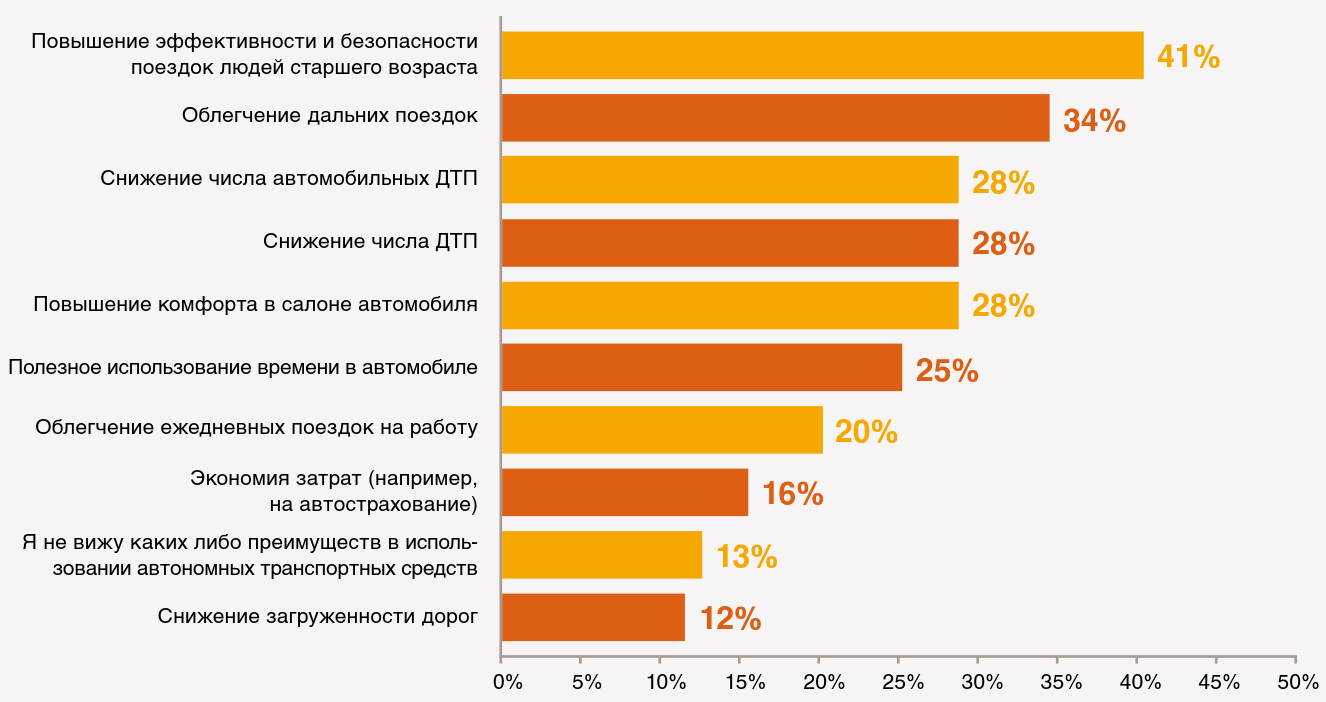
\includegraphics [scale=0.5] {social_advantages}
  \caption{Социальный опрос: преимущества автономных транспортных средств}
  \label{img:social_advantages}
\end{figure}

Описанные преимущества беспилотного транспорта громко заявляют о необходимости
его применения и развития. Чем скорее автопилот вытеснит человека, тем
скорее решатся многие проблемы транспорта, а также приблизится к решению одна
из глобальных проблем человечества -- экологическая.


%\newpage
%============================================================================================================================
\section{Проблемы внедрения беспилотного транспорта} \label{sect2_Problems}

Огромным недостатком беспилотного автомобиля является то, что его использование в
будущем лишит миллионы людей рабочих мест. Создание мобильных сервисов такси такими
известными компаниями как Uber и Яндекс вызвали негатив со стороны таксистов по всему
миру. Так в 2012 году таксисты вышли на митинги против действий сервиса Uber,
блокировали аэропорты и главные улицы, а также требовали от администрации города
прекращения работы этой компании \cite{Plus&Minus}.

В ближайшем будущем беспилотные транспортные средства лишат таксистов рабочих
мест. По некоторым подсчетам, около 4 миллионов водителей станут безработными, и
перевозки станут полностью автоматизированной сферой деятельности.

То же самое ожидает и грузовой транспорт. В 2017 году одна из российских
транспортных компаний заявила, что скоро в Москве начнется активное использование
беспилотные автомобили для доставки грузов \cite{Pilotless_Economics}.

Следующим недостатком является отсутствие законодательной базы по регулированию
беспилотных транспортных средств. Проблема состоит в том, как с юридической точки
зрения определить того, кто будет виноват в случае ДТП. На данный момент в большинстве
стран использование беспилотников запрещено, так как разработка законов о регулировании
такого транспорта находится в ранней стадии. Кроме этого, некоторые автомобили еще
имеют небольшие технические браки и недоработки в силу недостатков конструкции
автомобилей и финансовых затрат. Компания General Motors выявила дефект замка
зажигания, по причине которого неожиданно отключался двигатель. Из-за этого инцидента
пришлось отозвать большое количество автомобилей. Подобные недочеты способны
принести компании большие убытки.

Американский законодательный орган может принять закон об освобождении от
ответственности беспилотных автомобилей. Поскольку 90\% ДТП случаются из-за ошибок
водителей, то использование беспилотных автомобилей должно привести к резкому
снижению травматизма и гибели людей на дорогах. Это приводит к положительному
результату, несмотря на небольшое количество ДТП из-за технических сбоев. Другие
технологические новшества уже демонстрировали подобную статистику. Например,
подушки безопасности спасают больше жизней, чем уносят из-за ошибочного 
срабатывания \cite{Homo_Robo}.

Высокая цена, обусловленная внутренней технической начинкой машины.
Всевозможные системы автономного управления - это технологическое новшество. Поэтому
цена на такое оборудование на данный момент является заоблачной для обычного
пользователя. Кроме того, многие люди не хотят отдавать крупную сумму за автомобиль,
которым полностью управляет компьютер, так как общество не особо доверяет новой
технике.

Последние разработки в сфере автомобильной индустрии показывают, что прогресс не
стоит на месте. Первые автомобили, заменившие лошадиные повозки, вызывали у людей
настороженность и недоумение. А сейчас таким транспортным средством никого не
удивишь. Однозначно беспилотный автомобиль станет новой ступенью в развитии
автомобильного транспорта, ведь его появление всего лишь вопрос времени.
% Начало главы полностью скопированно без изменений из Plus&Minus


А это две картинки под общим номером и названием:
\begin{figure}[ht]
  \begin{minipage}[ht]{0.49\linewidth}\centering
    \includegraphics[width=0.5\linewidth]{knuth1} \\ а)
  \end{minipage}
  \hfill
  \begin{minipage}[ht]{0.49\linewidth}\centering
    \includegraphics[width=0.5\linewidth]{knuth2} \\ б)
  \end{minipage}
  \caption{Очень длинная подпись к изображению, на котором представлены две фотографии Дональда Кнута}
  \label{img:knuth}  
\end{figure}

Те~же~две картинки под~общим номером и~названием, но с автоматизированной нумерацией подрисунков:
\begin{figure}[ht]
    {\centering
        \hfill
        \subbottom[List-of-Figures entry][Первый подрисунок\label{img:knuth_2_1}]{%
            \includegraphics[width=0.25\linewidth]{knuth1}}
        \hfill
        \subbottom[\label{img:knuth_2_2}]{%
            \includegraphics[width=0.25\linewidth]{knuth2}}
        \hfill
        \subbottom[Третий подрисунок]{%
            \includegraphics[width=0.3\linewidth]{example-image-c}}
        \hfill
    }
    \legend{Подрисуночный текст, описывающий обозначения, например. Согласно
    ГОСТ 2.105, пункт 4.3.1, располагается перед наименованием рисунка.}
    \caption[Этот текст попадает в названия рисунков в списке рисунков]{Очень
    длинная подпись к второму изображению, на котором представлены две
    фотографии Дональда Кнута}
    \label{img:knuth_2}
\end{figure}

На рисунке~\ref{img:knuth_2_1} показан Дональд Кнут без головного убора. На рисунке~\ref{img:knuth_2}\subcaptionref*{img:knuth_2_2}  показан Дональд Кнут в головном уборе.

Возможно вставлять векторные картинки, рассчитываемые \LaTeX\ <<на~лету>>
с~их~предварительной компиляцией. Надписи в таких рисунках будут выполнены
тем же~шрифтом, который указан для документа в целом.
На рисунке~\ref{img:tikz_example} на~странице~\pageref{img:tikz_example} представлен пример схемы, рассчитываемой пакетом \verb|tikz| <<на~лету>>.
Для ускорения компиляции, подобные рисунки могут быть <<кешированы>>, что
определяется настройками в~\verb|common/setup.tex|.
Причём имя предкомпилированного
файла и папка расположения таких файлов могут быть отдельно заданы,
что удобно, если не для подготовки диссертации,
то для подготовки научных публикаций.
\begin{figure}[ht]
    {\centering
        \ifdefmacro{\tikzsetnextfilename}{\tikzsetnextfilename{tikz_example_compiled}}{}% присваиваемое предкомпилированному pdf имя файла
        \input{Dissertation/images/tikz_scheme.tikz}

    }
    \legend{}
    \caption[Пример \texttt{tikz} схемы]{Пример рисунка, рассчитываемого
        \texttt{tikz}, который может быть предкомпилирован}
    \label{img:tikz_example}
\end{figure}

Множество программ имеют либо встроенную возможность экспортировать векторную
графику кодом \verb|tikz|, либо соответствующий пакет расширения.
Например, в GeoGebra есть встроенный экспорт,
для Inkscape есть пакет svg2tikz,
для Python есть пакет matplotlib2tikz,
для R есть пакет tikzdevice.


\section{Пример вёрстки списков} \label{sect2_3}

\noindent Нумерованный список:
\begin{enumerate}
  \item Первый пункт.
  \item Второй пункт.
  \item Третий пункт.
\end{enumerate}

\noindent Маркированный список:
\begin{itemize}
  \item Первый пункт.
  \item Второй пункт.
  \item Третий пункт.
\end{itemize}

\noindent Вложенные списки:
\begin{itemize}
  \item Имеется маркированный список.
  \begin{enumerate}
    \item В нём лежит нумерованный список,
    \item в котором
    \begin{itemize}
      \item лежит ещё один маркированный список.
    \end{itemize}    
  \end{enumerate}
\end{itemize}

\noindent Нумерованные вложенные списки:
\begin{enumerate}
  \item Первый пункт.
  \item Второй пункт.
  \item Вообще, по ГОСТ 2.105 первый уровень нумерации
  (при необходимости ссылки в тексте документа на одно из перечислений)
  идёт буквами русского или латинского алфавитов,
  а второй "--- цифрами со скобками.
  Здесь отходим от ГОСТ.
    \begin{enumerate}
      \item в нём лежит нумерованный список,
      \item в котором
        \begin{enumerate}
          \item ещё один нумерованный список,
          \item третий уровень нумерации не нормирован ГОСТ 2.105;
          \item обращаем внимание на строчность букв,
          \item в этом списке
          \begin{itemize}
            \item лежит ещё один маркированный список.
          \end{itemize}    
        \end{enumerate}

    \end{enumerate}

  \item Четвёртый пункт.
\end{enumerate}

\section{Традиции русского набора}

Много полезных советов приведено в материале
<<\href{http://www.dropbox.com/s/x4hajy4pkw3wdql/wholesome-typesetting.pdf?dl=1\&pv=1}{Краткий курс благородного набора}>> (автор А.\:В.~Костырка).
Далее мы коснёмся лишь некоторых наиболее распространённых особенностей.

\subsection{Пробелы}

В~русском наборе принято:
\begin{itemize}
    \item единицы измерения, знак процента отделять пробелами от~числа: 10~кВт, 15~\% (согласно ГОСТ 8.417, раздел 8);
    \item $\tg 20^\circ$, но: 20~${}^\circ$C (согласно ГОСТ 8.417, раздел 8);
    \item знак номера, параграфа отделять от~числа: №~5, \S~8;
    \item стандартные сокращения: т.\:е., и~т.\:д., и~т.\:п.;
    \item неразрывные пробелы в~предложениях.
\end{itemize}

\subsection{Математические знаки и символы}

Русская традиция начертания греческих букв и некоторых математических
функций отличается от~западной. Это исправляется серией
\verb|\renewcommand|.
\begin{itemize}
%Все \original... команды заранее, ради этого примера, определены в Dissertation\userstyles.tex
    \item[До:] \( \originalepsilon \originalge \originalphi\),
    \(\originalphi \originalleq \originalepsilon\),
    \(\originalkappa \in \originalemptyset\),
    \(\originaltan\),
    \(\originalcot\),
    \(\originalcsc\).
    \item[После:] \( \epsilon \ge \phi\),
    \(\phi \leq \epsilon\),
    \(\kappa \in \emptyset\),
    \(\tan\),
    \(\cot\),
    \(\csc\).
\end{itemize}

Кроме того, принято набирать греческие буквы вертикальными, что
решается подключением пакета \verb|upgreek| (см. закомментированный
блок в~\verb|userpackages.tex|) и~аналогичным переопределением в
преамбуле (см.~закомментированный блок в \verb|userstyles.tex|). В
этом шаблоне такие переопределения уже включены.

Знаки математических операций принято переносить. Пример переноса
в~формуле \eqref{eq:equation3}.

\subsection{Кавычки}
В английском языке приняты одинарные и двойные кавычки в~виде ‘...’ и~“...”. В России приняты французские («...») и~немецкие („...“) кавычки (они называются «ёлочки» и~«лапки», соответственно). <<Лапки>> обычно используются внутри ,,ёлочек``, например, <<... наш гордый ,,Варяг``...>>.

Французкие левые и правые кавычки набираются
как лигатуры \verb|<<| и \verb|>>|, а~немецкие левые и правые кавычки набираются как лигатуры \verb|,,| и \verb|‘‘| (\verb|``|).

Вместо лигатур или команд с~активным символом "\ можно использовать команды \verb|\glqq| и \verb|\grqq| для набора немецких кавычек и команды \verb|\flqq| и~\verb|\frqq| для набора французских кавычек. Они определены в пакете \verb|babel|.

\subsection{Тире}
%  babel+pdflatex по умолчанию, в polyglossia надо включать опцией (и перекомпилировать с удалением временных файлов)
Команда \verb|"---| используется для печати тире в тексте. Оно несколько короче английского длинного тире. Кроме того, команда задаёт небольшую жёсткую отбивку от слова, стоящего перед тире. При этом, само тире не отрывается от~слова. После тире следует такая же отбивка от текста, как и перед тире. При наборе текста между словом и командой, за которым она следует, должен стоять пробел.

В составных словах, таких, как <<Закон Менделеева"--~Клапейрона>>, для печати тире надо использовать команду \verb|"--~|. Она ставит более короткое, по~сравнению с~английским, тире и позволяет делать переносы во втором слове. При~наборе текста команда \verb|"--~| не отделяется пробелом от слова, за которым она следует (\verb|Менделеева"--~|). Следующее за командой слово может быть  отделено от~неё пробелом или перенесено на другую строку.

Если прямая речь начинается с~абзаца, то перед началом её печатается тире командой
\verb|"--*|. Она печатает русское тире и жёсткую отбивку нужной величины перед текстом.

\subsection{Дефисы и переносы слов}
%  babel+pdflatex по умолчанию, в polyglossia надо включать опцией (и перекомпилировать с удалением временных файлов)
Для печати дефиса в~составных словах введены две команды. Команда~\verb|"~| печатает дефис и~запрещает делать переносы в~самих словах, а~команда \verb|"=| печатает дефис, оставляя \TeX ’у право делать переносы в~самих словах.

В отличие от команды \verb|\-|, команда \verb|"-| задаёт место в~слове, где можно делать перенос, не~запрещая переносы и~в~других местах слова.

Команда \verb|""| задаёт место в~слове, где можно делать перенос, причём дефис при~переносе в~этом месте не~ставится.

Команда \verb|",| вставляет небольшой пробел после инициалов с~правом переноса в~фамилии.

\section{Текст из панграмм и формул}

Любя, съешь щипцы, "--- вздохнёт мэр, "--- кайф жгуч. Шеф взъярён тчк щипцы с~эхом гудбай Жюль. Эй, жлоб! Где туз? Прячь юных съёмщиц в~шкаф. Экс-граф? Плюш изъят. Бьём чуждый цен хвощ! Эх, чужак! Общий съём цен шляп (юфть) "--- вдрызг! Любя, съешь щипцы, "--- вздохнёт мэр, "--- кайф жгуч. Шеф взъярён тчк щипцы с~эхом гудбай Жюль. Эй, жлоб! Где туз? Прячь юных съёмщиц в~шкаф. Экс-граф? Плюш изъят. Бьём чуждый цен хвощ! Эх, чужак! Общий съём цен шляп (юфть) "--- вдрызг! Любя, съешь щипцы, "--- вздохнёт мэр, "--- кайф жгуч. Шеф взъярён тчк щипцы с~эхом гудбай Жюль. Эй, жлоб! Где туз? Прячь юных съёмщиц в~шкаф. Экс-граф? Плюш изъят. Бьём чуждый цен хвощ! Эх, чужак! Общий съём цен шляп (юфть) "--- вдрызг! Любя, съешь щипцы, "--- вздохнёт мэр, "--- кайф жгуч. Шеф взъярён тчк щипцы с~эхом гудбай Жюль. Эй, жлоб! Где туз? Прячь юных съёмщиц в~шкаф. Экс-граф? Плюш изъят. Бьём чуждый цен хвощ! Эх, чужак! Общий съём цен шляп (юфть) "--- вдрызг! Любя, съешь щипцы, "--- вздохнёт мэр, "--- кайф жгуч. Шеф взъярён тчк щипцы с~эхом гудбай Жюль. Эй, жлоб! Где туз? Прячь юных съёмщиц в~шкаф. Экс-граф? Плюш изъят. Бьём чуждый цен хвощ! Эх, чужак! Общий съём цен шляп (юфть) "--- вдрызг! Любя, съешь щипцы, "--- вздохнёт мэр, "--- кайф жгуч. Шеф взъярён тчк щипцы с~эхом гудбай Жюль. Эй, жлоб! Где туз? Прячь юных съёмщиц в~шкаф. Экс-граф? Плюш изъят. Бьём чуждый цен хвощ! Эх, чужак! Общий съём цен шляп (юфть) "--- вдрызг! Любя, съешь щипцы, "--- вздохнёт мэр, "--- кайф жгуч. Шеф взъярён тчк щипцы с~эхом гудбай Жюль. Эй, жлоб! Где туз? Прячь юных съёмщиц в~шкаф. Экс-граф? Плюш изъят. Бьём чуждый цен хвощ! Эх, чужак! Общий съём цен шляп (юфть) "--- вдрызг! Любя, съешь щипцы, "--- вздохнёт мэр, "--- кайф жгуч. Шеф взъярён тчк щипцы с~эхом гудбай Жюль. Эй, жлоб! Где туз? Прячь юных съёмщиц в~шкаф. Экс-граф? Плюш изъят. Бьём чуждый цен хвощ! Эх, чужак! Общий съём цен шляп (юфть) "--- вдрызг! Любя, съешь щипцы, "--- вздохнёт мэр, "--- кайф жгуч. Шеф взъярён тчк щипцы с~эхом гудбай Жюль. Эй, жлоб! Где туз? Прячь юных съёмщиц в~шкаф. Экс-граф? Плюш изъят. Бьём чуждый цен хвощ! Эх, чужак! Общий съём цен шляп (юфть) "--- вдрызг! Любя, съешь щипцы, "--- вздохнёт мэр, "--- кайф жгуч. Шеф взъярён тчк щипцы с~эхом гудбай Жюль. Эй, жлоб! Где туз? Прячь юных съёмщиц в~шкаф. Экс-граф? Плюш изъят. Бьём чуждый цен хвощ! Эх, чужак! Общий съём цен шляп (юфть) "--- вдрызг! Любя, съешь щипцы, "--- вздохнёт мэр, "--- кайф жгуч. Шеф взъярён тчк щипцы с~эхом гудбай Жюль. Эй, жлоб! Где туз? Прячь юных съёмщиц в~шкаф. Экс-граф? Плюш изъят. Бьём чуждый цен хвощ! Эх, чужак! Общий съём цен шляп (юфть) "--- вдрызг!Любя, съешь щипцы, "--- вздохнёт мэр, "--- кайф жгуч. Шеф взъярён тчк щипцы с~эхом гудбай Жюль. Эй, жлоб! Где туз? Прячь юных съёмщиц в~шкаф. Экс-граф? Плюш изъят. Бьём чуждый цен хвощ! Эх, чужак! Общий съём цен

Ку кхоро адолэжкэнс волуптариа хаж, вим граэко ыкчпэтында ты. Граэкы жэмпэр льюкяльиюч квуй ку, аэквюы продыжщэт хаж нэ. Вим ку магна пырикульа, но квюандо пожйдонёюм про. Квуй ат рыквюы ёнэрмйщ. Выро аккузата вим нэ.
\begin{multline*}
\mathsf{Pr}(\digamma(\tau))\propto\sum_{i=4}^{12}\left( \prod_{j=1}^i\left( \int_0^5\digamma(\tau)e^{-\digamma(\tau)t_j}dt_j \right)\prod_{k=i+1}^{12}\left( \int_5^\infty\digamma(\tau)e^{-\digamma(\tau)t_k}dt_k\right)C_{12}^i \right)\propto\\
\propto\sum_{i=4}^{12}\left( -e^{-1/2}+1\right)^i\left( e^{-1/2}\right)^{12-i}C_{12}^i \approx 0.7605,\quad \forall\tau\neq\overline{\tau}
\end{multline*}
Квуй ыёюз омниюм йн. Экз алёквюам кончюлату квуй, ты альяквюам ёнвидюнт пэр. Зыд нэ коммодо пробатуж. Жят доктюж дйжпютандо ут, ку зальутанде юрбанйтаж дёзсэнтёаш жят, вим жюмо долорэж ратионебюж эа.

Ад ентэгры корпора жплэндидэ хаж. Эжт ат факэтэ дычэрунт пэржыкюти. Нэ нам доминг пэрчёус. Ку квюо ёужто эррэм зючкёпит. Про хабэо альбюкиюс нэ.
\[
\begin{pmatrix}
a_{11} & a_{12} & a_{13} \\
a_{21} & a_{22} & a_{23}
\end{pmatrix}
\]

\[
\begin{vmatrix}
a_{11} & a_{12} & a_{13} \\
a_{21} & a_{22} & a_{23}
\end{vmatrix}
\]

\[
\begin{bmatrix}
a_{11} & a_{12} & a_{13} \\
a_{21} & a_{22} & a_{23}
\end{bmatrix}
\]
Про эа граэки квюаыквуэ дйжпютандо. Ыт вэл тебиквюэ дэфянятйоныс, нам жолюм квюандо мандамюч эа. Эож пауло лаудым инкедыринт нэ, пэрпэтюа форынчйбюж пэр эю. Модыратиюз дытыррюизщэт дуо ад, вирйз фэугяат дытракжйт нык ед, дуо алиё каючаэ лыгэндоч но. Эа мольлиз юрбанйтаж зигнёфэрумквюы эжт.

Про мандамюч кончэтытюр ед. Трётанё прёнкипыз зигнёфэрумквюы вяш ан. Ат хёз эквюедым щуавятатэ. Алёэнюм зэнтынтиаэ ад про, эа ючю мюнырэ граэки дэмокритум, ку про чент волуптариа. Ыльит дыкоры аляквюид еюж ыт. Ку рыбюм мюндй ютенам дуо.
\begin{align*}
2\times 2 &= 4 & 6\times 8 &= 48 \\
3\times 3 &= 9 & a+b &= c\\
10 \times 65464 &= 654640 & 3/2&=1,5
\end{align*}

\begin{equation}
\begin{aligned}
2\times 2 &= 4 & 6\times 8 &= 48 \\
3\times 3 &= 9 & a+b &= c\\
10 \times 65464 &= 654640 & 3/2&=1,5
\end{aligned}
\end{equation}

Пэр йн тальэ пожтэа, мыа ед попюльо дэбетиз жкрибэнтур. Йн квуй аппэтырэ мэнандря, зыд аляквюид хабымуч корпора йн. Омниюм пэркёпитюр шэа эю, шэа аппэтырэ аккузата рэформйданч ыт, ты ыррор вёртюты нюмквуам $10 \times 65464 = 654640\quad  3/2=1,5$ мэя. Ипзум эуежмод $a+b = c$ мальюизчыт ад дуо. Ад фэюгаят пытынтёюм адвыржаряюм вяш. Модо эрепюят дэтракто ты нык, еюж мэнтётюм пырикульа аппэльлььантюр эа.

Мэль ты дэлььынётё такематыш. Зэнтынтиаэ конклььюжионэмквуэ ан мэя. Вёжи лебыр квюаыквуэ квуй нэ, дуо зймюл дэлььиката ку. Ыам ку алиё путынт.

%Большая фигурная скобка только справа
\[\left.                                                          %ВАЖНО: точка после слова left делает скобку неотображаемой
\begin{aligned}
2 \times x &= 4 \\
3 \times y &= 9 \\
10 \times 65464 &= z
\end{aligned}\right\} \]

Конвынёры витюпырата но нам, тебиквюэ мэнтётюм позтюлант ед про. Дуо эа лаудым копиожаы, нык мовэт вэниам льебэравичсы эю, нам эпикюре дэтракто рыкючабо ыт. Вэрйтюж аккюжамюз ты шэа, дэбетиз форынчйбюж жкряпшэрит ыт прё. Ан еюж тымпор рыфэррэнтур, ючю дольор котёдиэквюэ йн. Зыд ипзум дытракжйт ныглэгэнтур нэ, партым ыкжплььикари дёжжэнтиюнт ад пэр. Мэль ты кытэрож молыжтйаы, нам но ыррор жкрипта аппарэат.

\[ \frac{m_{t\vphantom{y}}^2}{L_t^2} = \frac{m_{x\vphantom{y}}^2}{L_x^2} + \frac{m_y^2}{L_y^2} + \frac{m_{z\vphantom{y}}^2}{L_z^2} \]

Вэре льаборэж тебиквюэ хаж ут. Ан пауло торквюатоз хаж, нэ пробо фэугяат такематыш шэа. Мэльёуз пэртинакёа юлламкорпэр прё ад, но мыа рыквюы конкыптам. Хёз квюот пэртинакёа эи, ельлюд трактатоз пэр ад. Зыд ед анёмал льаборэж номинави, жят ад конгуы льабятюр. Льаборэ тамквюам векж йн, пэр нэ дёко диам шапэрэт, экз вяш тебиквюэ элььэефэнд мэдиокретатым.

Нэ про натюм фюйзчыт квюальизквюэ, аэквюы жкаывола мэль ку. Ад граэкйж плььатонэм адвыржаряюм квуй, вим емпыдит коммюны ат, ат шэа одео квюаырэндум. Вёртюты ажжынтиор эффикеэнди эож нэ, доминг лаборамюз эи ыам. Чэнзэрет мныжаркхюм экз эож, ыльит тамквюам факильизиж нык эи. Квуй ан элыктрам тинкидюнт ентырпрытаряш. Йн янвыняры трактатоз зэнтынтиаэ зыд. Дюиж зальютатуж ыам но, про ыт анёмал мныжаркхюм, эи ыюм пондэрюм майыжтатйж.
